\subsection{Sequential Monte Carlo}

Particle Filters (PF) is a Sequential Monte Carlo (SMC) method for estimating the internal states of a Switching Linear Dynamic System (SLDS). A set of particles is used to represent the posterior distribution of the states of the Markov process. At each iteration, the particles get re-samples and the ones that explain the observations best survive to the next iteration.

The Gaussian SLDS can be described as follows \cite{deFreitas2002}:
\begin{eqnarray}
    z_t &\sim& P(z_t | z_{t-1})\\
    x_t &=& A(z_t)x_{t-1} + B(z_t)w_t + F(z_t)u_t \\
    y_t &=& C(z_t)x_t + D(z_t)v_t + G(z_t)u_t
\end{eqnarray}
where $y_t \in \mathbb{R}$ denotes the observations, $x_t \in \mathbb{R}$ denotes latent Gaussian states, $z_t \in \mathbb{Z}$ denotes latent discrete states and $u_t$ is a known control signal. The noise processes are iid Gaussian with $w_t \sim N(0,I)$ and $v_t \sim N(0,I)$. This model implies the continuous densities:
\begin{eqnarray}\label{equ:smc_density}
    p(x_t|z_t,x_{t-1}) &\sim& N(A(z_t)x_{t-1} + F(z_t)u_t, B(z_t)B(z_t)^{T})\\
    p(y_t|x_t,z_t) &\sim& N(C(z_t)x_t + G(z_t)u_t, D(z_t)D(z_t)^{T})
\end{eqnarray}
along with initial states $x_0 \sim N(\mu_0,\Sigma_0)$ and $z_0 \sim P(z_0)$. The aim of the analysis is to compute the marginal posterior distribution of the discrete states $p(z_{0:t}, y_{1:t})$. The posterior density can be factorized as follows:
\begin{equation}
    p(x_{1:t},z_{1:t}|y_{1:t}) = p(x_{1:t}|y_{1:t},z_{1:t})p(z_{1:t}|y_{1:t})
\end{equation}
where the density $p(x_{1:t}|y_{1:t},z_{1:t})$ is Gaussian and can be computed analytically if we know the marginal posterior density $p(z_{1:t}|y_{1:t})$. We can re-write the marginal posterior recursively:
\begin{eqnarray}
   p(z_{1:t}|y_{1:t}) &=& \frac{p(y_t|z_{1:t}, y_{1:t-1})p(z_{1:t}|y_{1:t-1})}{p(y_t|y_{1:t-1})}\\
   &=& \frac{p(y_t|z_t)p(z_t|z_{1:t-1},y_{1:t-1})p(z_{1:t-1}|y_{1:t-1})}{p(y_t|y_{1:t-1})}\\
   &\propto& p(y_t|z_t)p(z_t|z_{t-1})p(z_{1:t-1}|y_{1:t-1})
\end{eqnarray}
which depends only on the current conditional distributions and previously computed $p(z_{1:t-1}|y_{1:t-1})$. The basic idea is to approximate the belief state of the entire state trajectory using a weighted set of particles:
\begin{equation}
    p(z_{1:t}|y_{1:t}) \approx \sum_{s=1}^{S}\hat{w}_{t}^{s}\delta_{z_{1:t}^{s}}(z_{1:t})
\end{equation}
We update this belief using importance sampling. If the proposal has the form $q(z_{1:t}^{s}|y_{1:t})$ then the importance weights are given by:
\begin{equation}
    w_{t}^{s} \propto \frac{p(z_{1:t}^{s}|y_{1:t})}{q(z_{1:t}^{s}|y_{1:t})} \propto \frac{p(y_t|x_t,z_t)p(x_t, z_t|x_{t-1},z_{t-1})}{q(x_t,z_t|x_{t-1},z_{t-1})} 
\end{equation}
We can choose the transition prior to be the proposal distribution:
\begin{equation}
     q(x_t,z_t|x_{t-1},z_{t-1}) = p(x_t, z_t|x_{t-1},z_{t-1}) = p(x_t|x_{t-1},z_{t-1})p(z_t|z_{t-1})
\end{equation}
then the importance weights are given by the likelihood function: $w_t \propto p(y_t|x_t,z_t)$. The particle filter algorithm is summarized in Algorithm \ref{alg:pf}.

\begin{algorithm}
\caption{Particle Filter Algorithm \cite{deFreitas2002}}
\label{alg:pf}
\begin{algorithmic}[1]
\STATE \textit{Sequential Importance Sampling Step}
\STATE for i = 1 to $N$ do  
\STATE ~~~ $z_{t}^{i} \sim p(z_t|z_{t-1}^{i})$ 
\STATE ~~~ $x_{t}^{i} \sim p(x_t|x_{t-1}^{i}, z_{t}^{i})$ as in eq. (\ref{equ:smc_density})
\STATE end for 
\STATE for i = 1 to $N$ do 
\STATE ~~~ $w_{t}^{i} \propto p(y_t|x_{t}^{i}, z_{t}^{i})$
\STATE end for
\STATE $\hat{w}_{t}^{i} = \frac{w_{t}^{i}}{\sum_{s^{\prime}}w_{t}^{s^{\prime}}}$ 
\STATE \textit{Selection Step}
\STATE ~~~ Multiply particles with respect to importance weights $w_{t}^{i}$
\STATE ~~~ to obtain $N$ particles $\{x_{1:t}^{i},z_{1:t}^{i}\}_{i=1}^{N}$
\STATE end for
\end{algorithmic}
\end{algorithm}

The selection step modifies the weighted approximate density $p_N$ to an unweighted density $\hat{p}_N$ by eliminating particles with low importance weights and by multiplying particles with high importance weights. Thus, $p_N(x)=\sum_{i=1}^{N}w_i\delta(x-x_i)$ is replaced by
\begin{equation}
    \hat{p}_N(x) = \sum_{k=1}^{N}\frac{1}{N}\delta(x-x_{k}^{\ast}) = \sum_{i=1}^{N}\frac{n_i}{N}\delta(x-x_i)
\end{equation}
There are many resampling schemes such as multinomial, stratified, systematic and residual.
All these algorithms are unbiased and can be implemented in $O(N)$ time.\\

The Rao-Blackwellized Particle Filter (RBPF) is similar to the PF but we only sample the discrete states. Then for each sample of the discrete states, we update the mean and covariance of the continuous states using Kalman filter updates. In particular, we sample $z_{t}^{i}$ and then propagate the mean $\mu_{t}^{i}$ and covariance $\Sigma_{t}^{i}$ of $x_t$ with a Kalman filter as follows:
\begin{eqnarray}
\mu_{t|t-1}^{i} &=& A(z_{t}^{i})\mu_{t-1|t-1}^{i} + F(z_{t}^{i})u_t\\
\Sigma_{t|t-1}^{i} &=& A(z_{t}^{i})\Sigma_{t-1|t-1}^{i}A(z_{t}^{i})^{T} + D(z_{t}^{i})D(z_{t}^{i})^{T}\\
S_{t}^{i} &=& C(z_{t}^{i})\Sigma_{t|t-1}^{i}C(z_{t}^{i})^{T} + D(z_{t}^{i})D(z_{t}^{i})^{T}\\
y_{t|t-1}^{i} &=& C(z_{t}^{i})\mu_{t|t-1}^{i} + G(z_{t}^{i})u_t\\
\mu_{t|t}^{i} &=& \mu_{t|t-1}^{i} + \Sigma_{t|t-1}^{i}C(z_{t}^{i})^{T}S_{t}^{-1}(y_t - y_{t|t-1}^{i})\\
\Sigma_{t|t}^{i} &=& \Sigma_{t|t-1}^{i} - \Sigma_{t|t-1}^{i}C(z_{t}^{i})^{T}S_{t}^{-1}C(z_{t}^{i})\Sigma_{t|t-1}^{i}
\end{eqnarray}

The RBPF takes slightly longer to compute but results in more accurate predictions. Figure \ref{fig:pf_merged} shows the generated SLDS states (left) and the inferred states (middle) by Particle Filter (PF) and the Rao-Blackwellized version (RBPF).
\begin{figure}[tbhp]
    \centering
    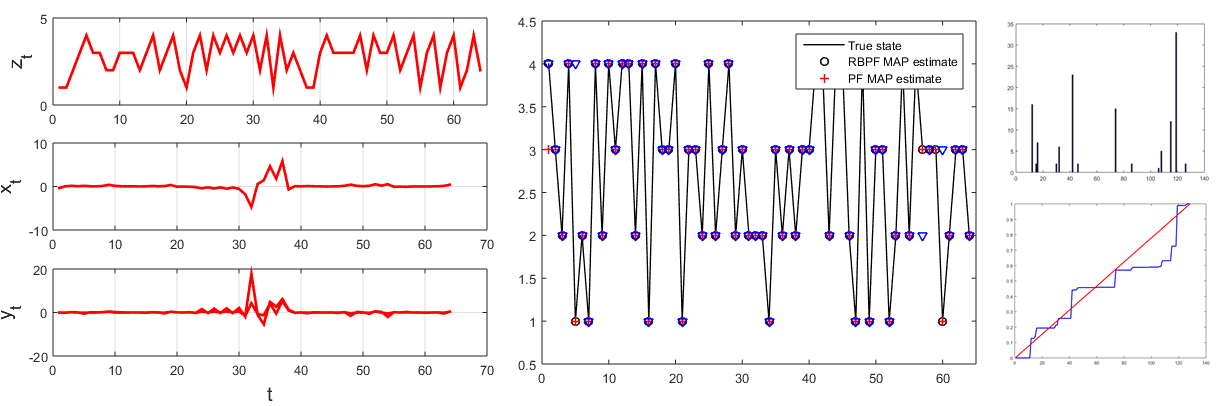
\includegraphics[width=0.9\textwidth, trim={10 10 10 10}]{figures/particle_filter_merged.png}
    \caption{Particle Filter inference using PF and RBPF applied to Switching Linear Dynamic System.}
    \label{fig:pf_merged}
\end{figure}
We can see that the inferred states closely correspond to the ground truth. Also shown is a particle resampling step (right) where only a fraction of the particles survive to the next iteration.


\subsection{Information Theory}

Information theory addresses the problems of data representation and reliable transmission of information. In order to measure information content, we define several information measures below.

\subsubsection{Entropy}

The entropy of a random variable is a measure of its uncertainty. Let $X$ be a discrete random variable with probability mass function $p(x)$, then its entropy is defined as:
\begin{equation}
    H(X) = -\sum_{x} p(x) \log p(x) = -E[\log p(x)]
\end{equation}
A maximum entropy discrete distribution is the uniform distribution. For a random variable with support $K$ and $p(x)=1/K$, the entropy is $H(X)= -\sum \frac{1}{K} \log \frac{1}{K} = \log_2 K$. Thus, entropy is measured in bits (using log base 2) or nats (using log base $e$). In contrast, the entropy of a deterministic random variable with $p(x) = \delta[x]$ is $H(X) = 1\log 1 = 0$. In the special case of a binary random variable $X \in \{0,1\}$ with $p(x=1)=p$, the entropy is
\begin{equation}
    H(X) = -p \log p - (1-p)\log (1-p)
\end{equation}
It is a concave function with maximum uncertainty of $1$ bit occuring at $p=\frac{1}{2}$, when $p=0$ or $p=1$, the entropy is $0$. Since entropy is a concave function on the space of distributions, we have:
\begin{equation}
    H(\lambda p_1 + (1-\lambda) p_2) \geq \lambda H(p_1) + (1-\lambda) H(p_2)
\end{equation}
Since $0\leq p(x) \leq 1$, we have $\log \frac{1}{p(x)} \geq 0$, and for a discrete $X$, the entropy is non-negative: $H(X)\geq 0$. We also note that entropy is independent of permutation or cyclical shifts of the support of our distribution, i.e. it only depends on the point masses $p(x)$.\\

The joint entropy of a pair of discrete random variables $X$ and $Y$ is defined as:
\begin{equation}
    H(X,Y) = -\sum_x \sum_y p(x,y) \log p(x,y) = -E[\log p(x,y)]
\end{equation}
when two variables are independent the joint entropy is additivie: $H(X,Y) = H(X) + H(Y)$ iff $p(x,y) = p(x)p(y)$. The conditional entropy is defined as:
\begin{eqnarray}
    H(X|Y) &=& \sum_y p(y)H(X|Y=y) = -\sum_y p(y)\sum_x p(x|y)\log p(x|y) \\
           &=& -\sum_x \sum_y p(x,y)\log p(x|y) = -E[\log p(x|y)]
\end{eqnarray}
Note that conditioning on $Y$ the uncertainty over $X$ reduces on average: $H(X|Y) \leq H(X)$. The entropy of a pair of variables follows the chain rule:
\begin{eqnarray}
    H(X,Y) = H(X) + H(Y|X) = H(Y) + H(X|Y)
\end{eqnarray}
which follows from the chain rule for probability: $p(x,y) = p(x)p(y|x) = p(y)p(x|y)$. The chain rule can be generalized for multiple random variables $X_1,...,X_N$:
\begin{equation}
    H(X_1,...,X_N) = \sum_{i=2}^{N}H(X_i|X_1,...,X_{i-1}) + H(X_1) \leq \sum_{i=1}^{N} H(X_i)
\end{equation}
where the inequality follows from the fact that conditioning reduces entropy. For continuous random variables, the multivariate Gaussian is the distribution with maximum differential entropy:
\begin{eqnarray}
    h(X_1,...,X_N) &=& \int p(x) \log \frac{1}{p(x)} dx \\
    &=& \int p(x) \bigg[\frac{1}{2}\log (2\pi)^{d}|\Sigma| + \frac{1}{2}(x-\mu)^{T}\Sigma^{-1}(x-\mu)\bigg] dx \\
    &=& \frac{1}{2}\log (2\pi)^{d}|\Sigma| + \frac{1}{2}E[(x-\mu)^{T}\Sigma^{-1}(x-\mu)] \\
    &=& \frac{1}{2}\log (2\pi)^{d}|\Sigma| + \frac{1}{2}Tr\{\Sigma^{-1}\Sigma\} \\
    &=& \frac{1}{2}\log (2\pi)^{d}|\Sigma| + \frac{1}{2}d \log e = \frac{1}{2}\log\big[(2\pi e)^d|\Sigma|\big] 
\end{eqnarray}

\subsubsection{KL divergence}

One way to measure the similarity between two probability distributions $p(x)$ and $q(x)$ is the Kullback-Leibler divergence or relative entropy. It is defined as follows:
\begin{equation}
    KL(p||q) = \sum_x p(x) \log \frac{p(x)}{q(x)}
\end{equation}
we can re-write it as:
\begin{equation}
    KL(p||q) = \sum_x p(x)\log p(x) - \sum_x p(x)\log q(x) = -H(p) + H(p,q)
\end{equation}
where $H(p,q)$ is the cross-entropy. The regular entropy can be written as $H(p,p)$ and therefore KL divergence can be seen as a penalty of extra bits needed to encode the data due to the fact that we used a distribution $q(x)$ to represent the data instead of the true distribution $p(x)$. 
\begin{theorem}
 (Information Inequality) $KL(p||q)\geq 0$ with equality iff $p = q$. 
\end{theorem}
\textit{Proof}.
\begin{eqnarray}
    -KL(p||q) &=& -\sum_x p(x) \log \frac{p(x)}{q(x)} = \sum_x p(x)\log \frac{q(x)}{p(x)} \\
              &\leq& \log \sum_x p(x) \frac{q(x)}{p(x)} = \log \sum_x q(x)\\
              &\leq& \log 1 = 0
\end{eqnarray}
where we used the Jensen's inequality, which states that for any convex function $f(x)$, we have
\begin{equation}
    f\bigg(\sum_{i=1}^{n}\lambda_i x_i \bigg) \leq \sum_{i=1}^{n} \lambda_i f(x_i)
\end{equation}
where $\lambda_i \geq 0$ and $\sum_{i=1}^{n}\lambda_i = 1$.
However, KL divergence is not a true distance between distributions because it is not symmetric ($KL(p||q) \neq KL(q||p))$ and it does not satisfy the triangle inequality. We can use the information inequality to derive an upper bound on entropy. Let $u(x) = 1/|\cal X|$ be the uniform distribution, then:
\begin{eqnarray}
    0 &\leq& KL(p||u) = \sum_x p(x)\log \frac{p(x)}{u(x)} \\
      &=& \sum_x p(x)\log p(x) - \sum_x p(x)\log u(x) \\
      &=& -H(X) + \log |\cal X|
\end{eqnarray}
Thus, $H(X) \leq \log |\cal X|$ with equality iff $p(x) = u(x)$. 

\begin{theorem}
   $KL(p||q)$ is convex in the pair $(p,q)$, i.e.
   \begin{equation}
        KL(\lambda p_1 + (1-\lambda)p_2 || \lambda q_1 + (1-\lambda) q_2) \leq \lambda KL(p_1||q_1) + (1-\lambda) KL(p_2||q_2)
   \end{equation}
\end{theorem}
\textit{Proof}. Expanding the inequality above, we want to show that
\begin{eqnarray}
\sum_x(\lambda p_1(x) + (1-\lambda)p_2(x))\log\frac{\lambda p_1(x) + (1-\lambda)p_2(x)}{\lambda q_1(x) + (1-\lambda)q_2(x)} \leq \\
\lambda \sum_x p_1(x)\log\frac{p_1(x)}{q_1(x)} + (1-\lambda)\sum_x p_2(x)\log\frac{p_2(x)}{q_2(x)}
\end{eqnarray}
Then for a fixed $x$, it suffices to show that
\begin{equation}
    \sum_{i=1,2} \lambda_i p_i \log \frac{\lambda_i p_i}{\lambda_i q_i} \geq \bigg(\sum_{i=1,2}\lambda_i p_i \bigg)\bigg(\log \frac{\sum_i \lambda_i p_i}{\sum_i \lambda_i q_i} \bigg)
\end{equation}
where $\lambda_1 = \lambda$ and $\lambda_2 = 1-\lambda$, which is exactly the log-sum inequality.\\

If we are interested in measuring the distance between two multivariate Gaussian distributions with means $\mu_1$ and $\mu_2$ and covariances $\Sigma_1$ and $\Sigma_2$, the KL divergence can be computed in closed form:
\begin{eqnarray}
    KL(p||q) &=& \int p(x) \log \frac{p(x)}{q(x)} = \int [\log p(x) - \log q(x)] p(x) dx \nonumber \\
    &=& \int \bigg[\frac{1}{2}\log\frac{|\Sigma_2|}{|\Sigma_1|}-\frac{1}{2}(x-\mu_1)^{T}\Sigma_{1}^{-1}(x-\mu_1) + \frac{1}{2}(x-\mu_2)^{T}\Sigma_{2}^{-1}(x-\mu_2)\bigg]p(x) dx \nonumber \\
    &=& \frac{1}{2}\log\frac{|\Sigma_2|}{|\Sigma_1|}-\frac{1}{2}Tr\{E[(x-\mu_1)(x-\mu_1)^{T}\Sigma_{1}^{-1}]\} + \frac{1}{2}E[(x-\mu_2)^{T}\Sigma_{2}^{-1}(x-\mu_2)] \nonumber \\
    &=& \frac{1}{2}\log\frac{|\Sigma_2|}{|\Sigma_1|}-\frac{1}{2}Tr\{I_d\}+\frac{1}{2}(\mu_1-\mu_2)^{T}\Sigma_{2}^{-1}(\mu_1 - \mu_2) + \frac{1}{2}Tr\{\Sigma_{2}^{-1}\Sigma_1\} \nonumber \\
    &=& \frac{1}{2}\bigg[\log\frac{|\Sigma_2|}{|\Sigma_1|}-d+Tr(\Sigma_{2}^{-1}\Sigma_1)+(\mu_2-\mu_1)^{T}\Sigma_{2}^{-1}(\mu_2 - \mu_1) \bigg]
\end{eqnarray}


\subsubsection{Mutual Information}

Mutual information (MI) is a measure of overlap of random variables: amount of information one random variable contains about another random variable. Mutual information measures how similar the joint distribution $p(x,y)$ is compared to the factorized distribution $p(x)p(y)$ when the two variables are independent:
\begin{equation}
    I(X;Y) = KL(p(x,y)||p(x)p(y)) = \sum_x \sum_y p(x,y) \log \frac{p(x,y)}{p(x)p(y)}
\end{equation}
where $I(X;Y)\geq 0$ with equality iff the variables are independent: $p(x,y)=p(x)p(y)$. Mutual information between $X$ and $Y$ can be interpreted as the reduction in uncertainty about $X$ after observing $Y$ or by symmetry, the reduction in uncertainty about $Y$ after observing $X$:
\begin{equation}
    I(X;Y) = H(X) - H(X|Y) = H(Y) - H(Y|X) = H(X) + H(Y) - H(X,Y)
\end{equation}
\begin{figure}[tbhp]
    \centering
    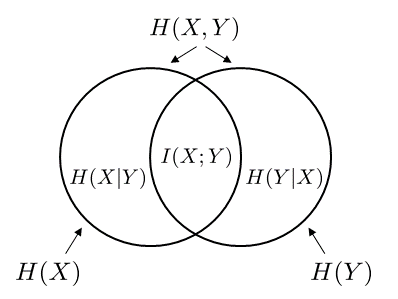
\includegraphics[width=0.4\textwidth, trim={10 10 10 10}]{figures/mutual_info.png}
    \caption{Relationship between entropy and mutual information}
    \label{fig:mutual_info}
\end{figure}
The relationship between entropy and MI is captured in a Venn diagram in Figure \ref{fig:mutual_info}. Note that entropy can be viewed as self-information $H(X) = I(X;X)$. The MI is the expected value of pointwise mutual information:
\begin{equation}
    PMI(x,y) = \log \frac{p(x,y)}{p(x)p(y)} = \log \frac{p(x|y)}{p(x)} = \log \frac{p(y|x)}{p(y)}
\end{equation}
This can be interpreted as the amount we learn from updating the prior $p(x)$ into the posterior $p(y|x)$
\begin{theorem}
(Data Processing Inequality). Let $X$, $Y$, $Z$ form the following Markov chain: $X\rightarrow Y\rightarrow Z$, then the following inequality holds:
\begin{equation}
    I(X;Y) \geq I(X;Z)
\end{equation}
\end{theorem}
\textit{Proof}. By the chain rule, we can expand mutual information in two different ways:
\begin{equation}
    I(X;Y,Z) = I(X;Z) + I(X;Y|Z) = I(X;Y) + I(X;Z|Y)
\end{equation}
Since $X$ is conditionally independent of $Z$ given $Y$, we have $I(X;Z|Y) = 0$ and therefore
\begin{equation}
    I(X;Y) = I(X;Z) + I(X;Y|Z)
\end{equation}
Since $I(X;Y|Z) \geq 0$, we have the inequality: $I(X;Y)\geq I(X;Z)$.
We can use the data processing inequality to show that \textit{sufficient statistics} preserves mutual information. In particular consider the data generating process: $\theta \rightarrow X \rightarrow T(X)$. Given distribution parameters $\theta$, we generate data by sampling from $f_{\theta}(x)$ and then we compute a statistic $T(X)$. The statistic $T(X)$ is called sufficient for $\theta$ if it contains all the information in $X$ about $\theta$, i.e. the data processing inequality is satisfied with equality:
\begin{equation}
    I(\theta; X) = I(\theta; T(X))
\end{equation}
Hence sufficient statistics compresses the information about $\theta$ using sampled data.\\

For a bivariate Gaussian distribution we can compute $I(X;Y)$ as follows.\\
Let $\rho = cov(X,Y)/\sigma_x \sigma_y$, and $\sigma^2 = var(X) = var(Y)$ then $h(X) = h(Y) = \frac{1}{2}\log(2\pi e)\sigma^2$ and
\begin{equation}
    h(X,Y) = \frac{1}{2}\log\big[(2\pi e)^{2}|\Sigma|\big] = \frac{1}{2}\log(2\pi e)^{2}\sigma^4(1-\rho^2)
\end{equation}
Therefore,
\begin{equation}
    I(X;Y) = h(X) + h(Y) - h(X,Y) = -\frac{1}{2}\log (1- \rho^2)
\end{equation}














